\chapter{Regret Matching}
\label{chapter:regret-matching}

\newcommand{\graphicsRM}[2]{
\begin{figure}[h]
    \resizebox{\textwidth}{!}{
    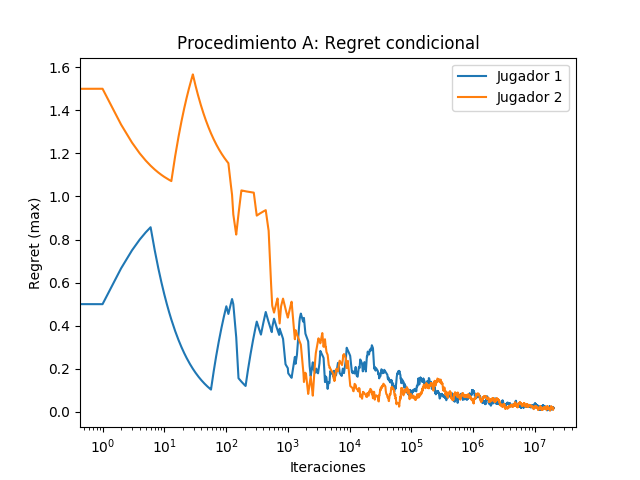
\includegraphics{graficas/regret-matching/#1/procedimiento-A.png}
    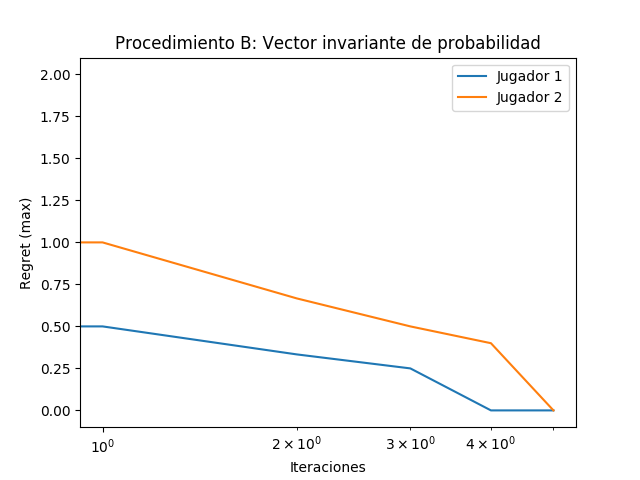
\includegraphics{graficas/regret-matching/#1/procedimiento-B.png} 
    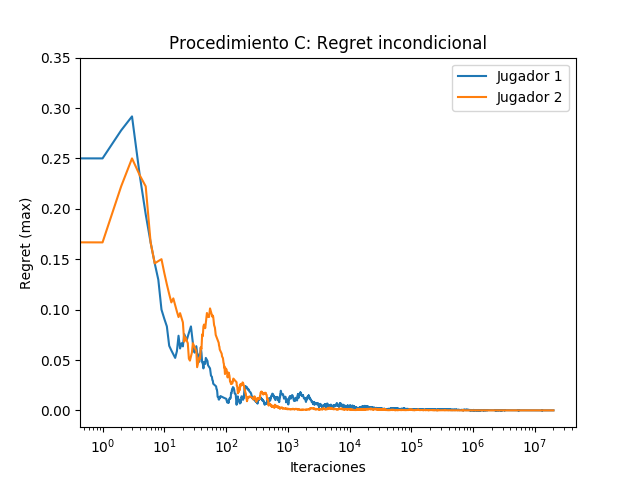
\includegraphics{graficas/regret-matching/#1/procedimiento-C.png}
    }
    \caption{Gráficas del \textit{regret} con respecto al número de iteraciones del juego #2.}
    \label{fig:regret-rm-#1}
\end{figure}
}

En la sección~\ref{section:equilibrio-correlacionado} se introdujo el concepto de equilibrio correlacionado (Definición~\ref{def:equilibrio-correlacionado}). Además, se afirma que el conjunto de equilibrios correlacionado es un conjunto simple. A continuación se describen tres procedimientos, dos de los cuales llevan a equilibrios correlacionados \cite{bib:correlated-equilibrium}.

\subsection*{Procedimiento A: Regret Condicional \cite{bib:correlated-equilibrium}}

Sea $\Gamma$ un juego en forma normal el cual es jugado repetidamente a través del tiempo $t = 1, 2, \ldots $. 
Sea $h_t = (s^\tau)_{\tau = 1}^t \in \prod_{\tau = 1}^{t} S$ la historia del juego al inicio del tiempo $t+1$; i.e., el $s^\tau$ es el perfil estratégico a tiempo $\tau$ que contiene las acciones realizadas por cada jugador. El jugador $i \in N$ elige la estrategia a utilizar a tiempo $t+1$ con una distribución de probabilidad $p_{t+1}^i \in \Delta(S_i)$, definida de la siguiente manera. Para cada par de estrategias $j, k \in S_i$, supongamos que el jugador $i$ remplaza la estrategia $j$ (cada vez que la jugó en el pasado) por la estrategia $k$. Luego, su ganancia a tiempo $1\leq \tau \leq t$ hubiera sido:
\begin{alignat}{1}
W_i^{\tau}(j,k)\ =\ 
\begin{cases}
u_i(k, s_{-i}^{\tau}) &\text{ si } s_i = j \,, \\
u_i(s^\tau) & \text{en otro caso.} 
\end{cases}
\end{alignat}

La diferencia resultante en el promedio de la función de pago, denotada con $D_i^t(j, k)$, para el jugador $i$ viene dada por \eqref{eq:diferencia-pago}. Por otra parte, la expresión \eqref{eq:regret} se puede interpretar como una medida de \say{arrepentimiento} del jugador $i$ de haber elegido la acción $j$ en vez de la acción $k$ en el pasado, y por lo tanto, dicha medida es denominada \textit{regret}.
\begin{alignat}{1}
\label{eq:diferencia-pago}
  D_i^t(j, k)\ 
    &=\ \frac{1}{t} \sum_{\tau = 1}^{t} W_i^{\tau}(j, k) - \frac{1}{t} \sum_{\tau = 1}^{t} u_i(s^{\tau})\ 
	=\ \frac{1}{t} \sum_{\substack{1\leq \tau \leq t \\s^\tau_i = j}} u_i(k, s_{-i}^{\tau}) - u_i(s^{\tau})\,, \\
\label{eq:regret}
R_i^t(j, k)\ &=\ [D_i^t(j, k)]^+\ =\ \max\{0, D_i^t(j, k)\} \,.
\end{alignat}

Fijemos un número $\mu > 0$ suficientemente grande. Sea $j \in S_i$ la última estrategia jugada por el jugador $i$, es decir $j = s_i^t$. Luego, la distribución de probabilidad $p_{t+1}^i \in \Delta(S_i)$ usada por el jugador $i$ a tiempo $t+1$ es definida como:
\begin{alignat}{1}
\label{eq:proc-A}
  \begin{cases}
    p_{t+1}^i(k)\ :=\  \frac{1}{\mu} R_i^t(j, k) & \text{ si $k \neq j$} \,, \\
    p_{t+1}^i(j)\ :=\ 1 - \sum_{k \in S_i, k \neq j} p_{t+1}^i(k) & \text{si $k=j$} \,.
  \end{cases}
\end{alignat}

La distribución inicial $p_{1}^i \in \Delta(S_i)$, a tiempo $t=1$, es elegida de forma arbitraria. Para cada tiempo $t$, sea $z_t \in \Delta(S)$ la distribución empírica de las $N$-tuplas jugadas hasta tiempo $t$, es decir:
$z_t(s) = \frac{1}{t} |\{1\leq\tau \leq t : s^{\tau} = s \}|$. El siguiente teorema enuncia que el procedimiento arriba descrito produce un equilibrio correlacionado.

\begin{theorem}[{\cite[p.~1131]{bib:correlated-equilibrium}}]
\label{theo:conv-proc-A}
Si cada jugador juega de acuerdo al procedimiento descrito por \eqref{eq:proc-A}, entonces la distribución empírica del juego $z_t$ converge (a.s.) cuando $t \rightarrow \infty$ al conjunto de equilibrios correlacionado del juego $\Gamma$.\footnote{Convergencia a.s.\ (almost sure) indica que el conjunto de  secuencias $\{z_t\}_t$ para las cuales la convergencia no se cumple es un conjunto de probabilidad 0.}
\end{theorem}

En el procedimiento descrito cada jugador tiene dos opciones en cada período: continuar jugando con la última estrategia, o cambiarla por otra estrategia cuyas probabilidades son proporcionales a cuanto mayor hubiese sido su ganancia acumulada si hubiese hecho ese cambio en el pasado. El procedimiento planteado es simple, tanto de entender y explicar, como de implementar. Además en cada período no sólo se elige la mejor respuesta, todas las respuestas mejores a la actual pueden ser escogidas con probabilidades que son proporcionales a sus ganancias aparentes (medidas por el \textit{regret}). Este tipo de procedimientos son llamados procedimientos de \textit{Regret Matching}. Por último, el procedimiento tiene inercia: la estrategia jugada previamente importa, siempre hay una probabilidad positiva de continuar jugando la misma estrategia, por lo tanto, sólo se cambiará de estrategia si hay una razón para hacerlo.

El \textit{regret} juega un papel importante en la elección de la siguiente distribución de probabilidad, lo cual conlleva a la siguiente pregunta: ?`Cuál es la relación entre los \textit{regrets} y el equilibrio correlacionado? Una condición necesaria y suficiente para que la distribución empírica converja al conjunto de equilibrio correlacionado es que todos los \textit{regrets} converjan a cero (Teorema \ref{theo:no-regret}).

\begin{theorem}[{\cite[p.~1133]{bib:correlated-equilibrium}}]
\label{theo:no-regret}
Sea $(s_t)_{t = 1, 2, ...}$ una secuencia de juegos de $\Gamma$.
Entonces, $R_i^t(j, k)$ converge a $0$ para cada $i$ y cada $j, k \in S_i$, con $j \neq k$, si y sólo si la secuencia de distribuciones empíricas $z_t$ converge al conjunto de equilibrio correlacionado.
\end{theorem}

\subsection*{Procedimiento B: Vector Invariante de Probabilidad}

Este procedimiento es una variación del anterior. Sin embargo, a tiempo $t+1$ las probabilidades de transición de la estrategia utilizada por el jugador $i$ son determinadas por la matriz estocástica (derecha) $M^i_t$ definida en \eqref{eq:proc-A}; i.e., $M^i_t(j,k)=\frac{1}{\mu}R^t_i(j,k)$ si $k\neq j$, y $M^i_t(j,j)=1-\frac{1}{\mu}\sum_{k\in S_i,k\neq j} R^t_i(j,k)$ si $k=j$ \cite[p.~1133]{bib:correlated-equilibrium}.

Considere un vector (fila) invariante de probabilidad $q^i_t$ (dicho vector siempre existe), donde $q^i_t\in \Delta(S_i)$, para la matriz $M^t$. Es decir, $q^i_t$ satisface $q^i_t \times M^i_t = q^i_t$, i.e., para todo $j$:
\begin{alignat}{1}
\label{eq:def-inv-vector}
  q^i_t(j)\ 
    =\ \sum_{k\in S_i} q^i_t(k) M^i_t(k,j)\ 
    =\ \bigg[\sum_{k \in S_i, k \neq j} q^i_t(k)\frac{1}{\mu}R^t_i(k,j)\bigg] + q_i^t(j)\biggl[1 - \frac{1}{\mu}\sum_{k \in S_i, k \neq j} R^t_i(j,k)\biggr]\,.
\end{alignat}

\begin{theorem}[{\cite[p.~1133]{bib:correlated-equilibrium}}]
\label{theo:def-proc-B}
Sea $R_t^i(j, j) = 0$. El vector $q_t^i$, definido en \ref{eq:def-inv-vector}, cumple que:
\begin{alignat}{1}
\label{eq:proc-B}
q^i_t(j)\sum_{k \in S_i} R^t_i(j,k)\ =\ \sum_{k \in S_i} q_t^i(k)R_i^t(k,j) \,.
\end{alignat}
\end{theorem}

\begin{theorem}[{\cite[p.~1133]{bib:correlated-equilibrium}}]
\label{theo:conv-proc-B}
Supongamos que a cada período $t+1$, el jugador $i$ elige las estrategias acorde a un vector de distribución de probabilidad $q_t^i$ que satisface \eqref{eq:proc-B}. Entonces, $R^i_t(j, k)$ converge a cero (a.s.) para todo $j, k \in S_i$ con $j \neq k$.
\end{theorem}

\subsection*{Procedimiento C: Regret Incondicional}

El tercer procedimiento no conduce necesariamente a un equilibrio correlacionado. Sin embargo es considerado \say{universalmente} consistente (Definición \ref{def:proc-univ-consistente}). En este procedimiento, el pago promedio del jugador $i$, en el límite, no es peor al pago si él hubiese jugado cualquier estrategia constante $k$, para todo $\tau \leq t$.

\begin{definition}[{\cite[p.~1139]{bib:correlated-equilibrium}}]
\label{def:proc-univ-consistente}
Un procedimiento adaptativo es \textbf{universalmente consistente} para el jugador $i$ si:
\begin{alignat}{1}
	\limsup_{t \rightarrow \infty } \left[ \max_{k \in S_i} \frac{1}{t} \sum_{\tau = 1}^{t} u_i(k, s_{-i}^{\tau}) - \frac{1}{t} \sum_{\tau = 1}^{t} u_i(s_{\tau}) \right]\ \leq\ 0\quad (a. s.) \,.
\end{alignat}
\end{definition}
El procedimiento es definido a continuación. A tiempo $t$, definimos
\begin{alignat}{1}
D_i^t(k)\ &=\ \frac{1}{t} \sum_{\tau = 1}^{t} u_i(k, s_{-i}^{\tau}) - u_i(s_{\tau}) \,, \\
\label{eq:diferencia-pago-ri}
R_i^t(k)\ &=\ [D_i^t(k)]^+\ =\ \max\{0, D_i^t(k)\} \,.
\end{alignat}
Luego, la distribución de probabilidad a tiempo $t+1$, $p_{t+1}^i \in \Delta(S_i)$, es definida como sigue:
\begin{alignat}{1}
\label{eq:proc-C}
  p_{t+1}^i(k)\ =\ \frac{R_i^t(k)}{\sum_{k'\in S_i} R_i^t(k')}
\end{alignat}
si el denominador es positivo, y de forma arbitraria en caso contrario. Note que las probabilidades son elegidas de forma proporcional a $R_i^t(k)$ que será denominado \textit{regret} incondicional (en contraste al \textit{regret} condicional definido previamente).

\begin{theorem}[{\cite[p.~1139]{bib:correlated-equilibrium}}]
\label{theo:conv-proc-C}
El procedimiento adaptativo definido en \eqref{eq:proc-C} es universalmente consistente para el jugador $i$.
\end{theorem}

\section{Regret Matching y Equilibrio de Nash}

?`Bajo qué condiciones se puede garantizar que un procedimiento universalmente consistente conduzca a un equilibrio de Nash? El Teorema~\ref{theo:UC-EN} permite concluir que en juegos de dos jugadores de suma cero, si un procedimiento es universalmente consistente, su distribución empírica llevará a un equilibrio de Nash (si $\mathcal{A}$ es un conjunto se utilizará $|\mathcal{A}|$ para denotar su cardinalidad).

\begin{theorem}
\label{theo:UC-EN}
Sea $\Gamma$ un juego de dos jugadores de suma cero y sea $(s^t)_{t=1,2,..., T}$ una secuencia de juegos de $\Gamma$, tales que, para todo $s_i \in S_i$, para todo $i \in {1, 2}$:
\begin{alignat}{1}
\frac{1}{T}\sum_{t = 1}^{T}u_i(s_i, s_{-i}^t) - \frac{1}{T} \sum_{t = 1}^T u_i(s^t)\ \leq\ \varepsilon
\end{alignat}
para algún $\varepsilon > 0$. Sea $\bar{\sigma}^T = (\bar{\sigma_1}^T, \bar{\sigma_2}^T)$, donde:
\begin{alignat}{1}
\bar{\sigma}_i^T(s_i)\ =\ \frac{|\{ t \leq T : s_i^t = s_i\}|}{T} \,,
\end{alignat}
es decir, $\bar{\sigma}^T$ es la distribución empírica de probabilidad, note que $|\{ t \leq T : s_i^t = s_i\}|$ es igual al número de veces que se eligió $s_i$ hasta el tiempo $T$. Entonces, $\bar{\sigma}^T$ es un $2\varepsilon$-equilibrio de Nash.
\end{theorem}

Por otra parte, los procedimientos A y B también son universalmente consistentes (corolario del Teorema~\ref{theo:a-b-universalmente-consistentes}), por lo que los tres procedimientos pueden ser utilizados para calcular una aproximación de un equilibrio de Nash en cualquier juego de dos jugadores de suman cero.

\begin{theorem}
\label{theo:a-b-universalmente-consistentes}
En un procedimiento adaptativo de \textit{Regret Matching}, si el \textit{regret} condicional converge a $0$, entonces el procedimiento es universalmente consistente.
\end{theorem}

\section{Evaluación Empírica de Regret Matching}

Los algoritmos propuestos fueron probados en 4 juegos diferentes en forma normal: \textit{matching pennies}, piedra, papel y tijera, ficha vs. dominó, y coronel Blotto. Todos estos juegos son de dos jugadores y, debido a que los algoritmos son universalmente consistentes, pueden ser utilizados para encontrar un equilibrio de Nash en cada uno de ellos. Además, es suficiente con definir el pago para el primer jugador para que el juego esté bien definido. 

Por otra parte, un equilibro de Nash en juegos de dos jugadores de suma cero puede modelarse como un problema de programación lineal \cite[pp.~228-233]{bib:pl-chvatal} (ver Apéndice \ref{apex:chapter:programacion-lineal}) y resolverse mediante procedimientos destinados para esto. Esto nos permite encontrar por otro procedimiento un equilibrio de Nash para juegos suficientemente pequeños, y así verificar la correctitud de los algoritmos de \emph{Regret Matching}. 

Cada uno de los juegos es descrito mediante sus reglas y, cuando sea factible, mostraremos la matriz de pagos explícitamente. Los problemas de programación lineal que permiten obtener un equilibrio de Nash en cada juego se encuentran en el Apéndice \ref{apex:chapter:programacion-lineal}.

La implementación fue realizada en el lenguaje C++ utilizando la librería estándar y una librería adicional llamada \textit{Eigen} \cite{bib:eigen} para factorizar matrices y resolver sistemas de ecuaciones. También se implementó una clase para encontrar un equilibrio de Nash mediante el algoritmo de \textit{Regret Matching}. En cada iteración del algoritmo, la actualización de las estrategias depende de cada procedimiento según las fórmulas propuestas anteriormente. La evaluación experimental de estos algoritmos se realizó en una máquina personal con las siguientes características: procesador Intel\textsuperscript{\textregistered} Core\textsuperscript{\texttrademark} i5-8250U \makeatletter{@} 1.60GHz, 8CPUs y 8GB de memoria. RAM.

Cada procedimiento fue probado $10$ veces para cada juego, finalizando cada ejecución al obtener un regret máximo menor a 0,005.  Para evaluar la convergencia se midió el tiempo necesario para alcanzar el \textit{regret} deseado y el número de iteraciones. Por cada juego se muestra una tabla con los resultados obtenidos que incluye para cada uno de los procedimientos, la ganancia esperada para el primer jugador al utilizar la estrategia obtenida en la última corrida del algoritmo ($u({\sigma})$) y la explotabilidad ($\varepsilon_{\sigma}$) de dicha estrategia, así como también el promedio sobre las $10$ ejecuciones del algoritmo del tiempo de ejecución en segundos ($T$), el número de iteraciones ($I$) y el tiempo por iteración ($T/I$). También se muestra las gráficas del \textit{regret} con respecto al número de iteraciones de cada uno de los procedimientos. Estas gráficas son mostradas con una escala logarítmica en el eje $x$ para apreciar mejor los resultados. En el Apéndice \ref{apex:chapter:experimentos-rm} se muestran tablas con resultados adicionales en cada una de las corridas.

\subsection*{Matching Pennies}

En este juego cada jugador tiene una moneda y selecciona cara o sello de forma secreta. Si las elecciones son iguales gana el jugador $1$, en caso contrario gana el jugador $2$. La matriz de pagos de este juego se muestra en la Tabla \ref{table:pagos-matching-pennies}.
\begin{table}[h]
\begin{center}
\caption[Tabla de pagos del juego matching pennies]{Tabla de pagos del juego \textit{matching pennies}.}
\label{table:pagos-matching-pennies}
\begin{tabular}{ c | c | c |}
 \multicolumn{1}{c}{} & \multicolumn{1}{c}{cara} & \multicolumn{1}{c}{sello}  \\ \cline{2-3}
 cara  &  1 & -1 \\ \cline{2-3}
 sello & -1 &  1 \\ \cline{2-3}
\end{tabular}
\end{center}
\end{table}

El problema de programación lineal es presentado en la Ecuación~\ref{apex:eq:pl-matching-pennies} (Apéndice~\ref{apex:chapter:programacion-lineal}), cuya solución primal y dual vienen dadas por la Ecuación \ref{eq:nash-matching-pennies}. Luego, el equilibrio de Nash se obtiene cuando ambos jugadores eligen cara o sello con probabilidad $\frac{1}{2}$ y el valor del juego es igual a $0$.
\begin{alignat}{1}
\label{eq:nash-matching-pennies}
(z^*, x_1^*, x_2^*)\ =\ (w^*, y^*_1, y^*_2)\ =\ \left(0, \frac{1}{2}, \frac{1}{2} \right) \,.
\end{alignat}

La Tabla~\ref{table:resultados-rm-matching-pennies} muestra los resultados experimentales obtenidos. Note que la explotabilidad siempre es menor que $0,008$. La Figura~\ref{fig:regret-rm-matching-pennies} muestra el \textit{regret} con respecto al número de iteraciones en cada juego. Se observa como el \textit{regret} tiende a cero en cada una de las gráficas.
 
\begin{table}[t]
\caption{Resultados experimentales del juego matching pennies.}
\label{table:resultados-rm-matching-pennies}
\centering
\begin{tabular}{l r r r}
    \toprule
    & \multicolumn{1}{c}{A} & \multicolumn{1}{c}{B} & \multicolumn{1}{c}{C} \\ \midrule
    Ganancia esperada $u(\sigma)$             &     0,000 &      0,000 &      0,000 \\
    Explotabilidad $\varepsilon_{\sigma}$     &         0,006 &      0,006 &      0,008 \\
    Tiempo $T$                                &        10,276 &      0,777 &      0,042 \\
    Iteraciones $I$                           & 3.892.550,4   & 25.616,6   & 16.260,5   \\
    $T/I$                                     & $2,64{\times}10^{-6}$ & $3,03{\times}10^{-5}$ & $2,58{\times}10^{-6}$ \\
    \bottomrule
\end{tabular}
\end{table}
\graphicsRM{matching-pennies}{matching pennies}

\subsection*{Piedra, Papel o Tijera}

Este juego es descrito en el Capítulo~\ref{chapter:forma-normal} y su matriz de pago se muestra en la Tabla \ref{table:pago-RPS}. El problema de programación lineal asociado se encuentra en la Ecuación~\ref{apex:eq:pl-RPS} y su solución (primal y dual) es:
\begin{alignat}{1}
(z^*, x_1^*, x_2^*, x_3^*)\ =\ (w^*, y_1^*, y_2^*, y_3^*)\ =\  \left(0, \frac{1}{3}, \frac{1}{3}, \frac{1}{3}\right) \,,
\end{alignat}
Luego, el equilibrio de Nash se obtiene cuando ambos jugadores eligen cada una de las acciones con probabilidad igual a $\frac{1}{3}$ y el valor del juego es igual a $0$. Es importante destacar que en todo juego simétrico el valor del juego es $0$ y las estrategias óptimas son iguales para ambos jugadores.

La Tabla~\ref{table:resultados-rm-RPS} muestra el resumen de los resultados para piedra, papel o tijera. Note que la explotabilidad siempre es menor o igual que 0,01. La gráfica~\ref{fig:regret-rm-RPS} muestra el \textit{regret} con respecto al número de iteraciones para cada uno de los procedimientos.

\begin{table}[t]
\caption{Resultados experimentales del juego piedra, papel o tijera.}
\label{table:resultados-rm-RPS}
\centering
\begin{tabular}{l r r r}
    \toprule
    & \multicolumn{1}{c}{A} & \multicolumn{1}{c}{B} & \multicolumn{1}{c}{C} \\ \midrule
    Ganancia esperada $u(\sigma)$         & -0,000012 & 0,000004 & 0,000022 \\
    Explotabilidad $\varepsilon_{\sigma}$ &  0,006 & 0,010 & 0,009 \\
    Tiempo $T$                            & 12,198 & 0,345 & 0,049 \\
    Iteraciones $I$                       & 4.519.054,1 & 6.601,3 &  19.321,1 \\
    $T/I$                                 & $2,70{\times}10^{-6}$ & $5,23{\times}10^{-5}$ & $2,54{\times}10^{-6}$\\
    \bottomrule
\end{tabular}
\end{table}
\graphicsRM{RPS}{piedra, papel o tijera}

\subsection*{Ficha vs.\ Dominó}

En este juego cada jugador tiene un tablero de tamaño $2\times 3$. El primer jugador tiene una ficha de dominó que puede colocar de $7$ formas diferentes. Cada una de las formas es mostrada en la Figura~\ref{fig:posiciones-domino}, con su respectiva etiqueta. El segundo jugador posee una ficha que ocupa una única casilla de su tablero y la ubica en una de las $6$ casillas, las cuales se numeran en la Figura~\ref{fig:posiciones}. Luego se superponen los tableros y si la ficha es cubierta por el dominó entonces el segundo jugador gana, en caso contrario gana el primer jugador \cite[p. 237]{bib:pl-chvatal}. La matriz de pagos de este juego se muestra en la Tabla \ref{table:pagos-domino}.

\begin{figure}[t]
\centering

\includegraphics[width=0.25\textwidth]{figuras/posiciones.png}
\caption{Posibles posiciones de la ficha del segundo jugador en el juego ficha vs.\ dominó.}
\label{fig:posiciones}
\end{figure}

\begin{figure}[t]
\centering

\includegraphics[width=\textwidth]{figuras/posiciones-domino.png}
\caption{Posibles posiciones de la ficha de dominó que representas las acciones del primer jugador en el juego ficha vs.\ dominó.}
\label{fig:posiciones-domino}
\end{figure}

\begin{table}[t]
\begin{center}
\caption{Matriz de pagos del juego ficha vs.\ dominó.}
\label{table:pagos-domino}
\begin{tabular}{ c | c | c | c | c | c | c |}
\multicolumn{1}{c}{}  &  \multicolumn{1}{c}{1} &  \multicolumn{1}{c}{2} & \multicolumn{1}{c}{3} & \multicolumn{1}{c}{4} & \multicolumn{1}{c}{5} & \multicolumn{1}{c}{6} \\ \cline{2-7}
A & -1 & -1 &  1 &  1 &  1 &  1 \\ \cline{2-7}
B &  1 &  1 &  1 & -1 & -1 &  1 \\ \cline{2-7}
C &  1 & -1 & -1 &  1 &  1 &  1 \\ \cline{2-7}
D &  1 &  1 &  1 &  1 & -1 & -1 \\ \cline{2-7}
E & -1 &  1 &  1 & -1 &  1 &  1 \\ \cline{2-7}
F &  1 & -1 &  1 &  1 & -1 &  1 \\ \cline{2-7}
G &  1 &  1 & -1 &  1 &  1 & -1 \\ \cline{2-7}
\end{tabular}
\end{center}
\end{table}

El problema de programación lineal asociado se encuentra en la Ecuación~\ref{apex:eq:pl-domino}. Este problema no tiene solución única (lo que implica que el juego no tiene un equilibrio de Nash único), una solución (primal y dual) viene dada por:

\begin{alignat}{1}
(z^*, x^*_1, x^*_2, x^*_4, x^*_5, x^*_6, x^*_6, x^*_7)\ =\ \left(\frac{1}{3}, \frac{1}{3}, \frac{1}{3}, 0, 0, 0, 0, \frac{1}{3}\right) \,, \\
(w^*, y^*_1, y^*_2, y^*_3,  y^*_4, y^*_5, y^*_6)\ =\ \left(\frac{1}{3}, \frac{1}{3}, 0, \frac{1}{3}, 0, \frac{1}{3}, 0\right) \,.
\end{alignat}

Esta solución corresponde a la estrategia en la que el jugador $1$ elige las posiciones A, B y G con probabilidad $\frac{1}{3}$ cada una, y el jugador $2$ elige las posiciones $1$, $3$, y $5$ con probabilidad $\frac{1}{3}$ cada una. Además, el valor del juego es igual a $\frac{1}{3}$. La Tabla~\ref{table:resultados-rm-domino} muestra el resumen de los resultados experimentales. Note que la máxima explotabilidad es igual a 0,01. Por otra parte, la Figura~\ref{fig:regret-rm-domino} muestra el \textit{regret} con respecto al número de iteraciones de este juego, donde se observa la convergencia del \textit{regret} en cada una de ellas.

\begin{table}[h]
\caption{Resultados Experimentales del juego ficha vs.\ dominó.}
\label{table:resultados-rm-domino}
\centering
\begin{tabular}{l r r r}
    \toprule
    & \multicolumn{1}{c}{A} & \multicolumn{1}{c}{B} & \multicolumn{1}{c}{C} \\ \midrule
    Ganancia esperada $u(\sigma)$ & 0,333 & 0,334 & 0,334  \\
    Explotabilidad $\varepsilon_{\sigma}$ & 0,010 & 0,007 & 0,004 \\
    Tiempo $T$ & 319,179 & 11,275 & 0,237  \\
    Iteraciones $I$ & 108.319.272,4 & 75.250,2 & 84.318,5 \\
    $T/I$ & $2,95 {\times} 10^{-6}$ & $1,50 {\times} 10^{-4}$ & $2,81 {\times} 10^{-6}$ \\
    \bottomrule
\end{tabular}
\end{table}
\graphicsRM{domino}{ficha vs.\ dominó}
 
\subsection*{Coronel Blotto}

En este juego cada uno de los jugadores tiene $S$ soldados en total que debe ubicar en $N$ campos de batallas. Cada soldado debe ser asignado a un único campo, pero cualquier número de soldados puede ser colocado en cualquier campo, incluyendo cero. Un jugador obtiene un campo de batalla si asigna más soldados que su oponente en ese campo de batalla. El juego es ganado por el jugador que obtenga un mayor número de campos y su pago es igual a la diferencia entre el número de campos obtenidos por cada uno de los jugadores \cite{bib:blotto-game}.

Formalmente el juego puede ser descrito de la siguiente manera. Cada jugador debe elegir $N$ números enteros, digamos $(a_1, a_2, ..., a_N)$ y $(b_1, b_2, ..., b_N)$, para el jugador $1$ y $2$ respectivamente, tales que $a_1 + a_2 + ... + a_N = S$ y $b_1 + b_2 + ... + b_N = S$, con $N < S$, donde $a_i$ y $b_i$ es la cantidad de soldados ubicados el $i$-ésimo campo por el primer y segundo jugador, respectivamente. La ganancia del jugador $1$ viene dada por:
\begin{alignat}{1}
|\{ 1 \leq i \leq N : a_i > b_i\}| - |\{ 1 \leq i \leq N : a_i < b_i\}| \,.
\end{alignat}

Este juego depende de dos parámetros: el número de soldados $S$ y el número de campos de batallas $N$, por lo que la matriz de pagos no es constante y por eso no es presentada como en los juegos anteriores. La matriz para un juego con $S$ soldados y $N$ es una matriz cuadrada de tamaño $\binom{N+S-1}{S-1}$.

En este juego es necesario generar la matriz de pagos dependiendo de los parámetros. Para esto se creó un programa que dado el número de campos de batalla ($N$) y el número de soldados ($S$), se generan todas las posibles distribuciones de cada uno de los jugadores mediante un algoritmo de \textit{backtracking}, y calcula el pago para cada juego posible, obteniendo como salida del programa la matriz deseada. De esta forma se generó la matriz de pagos para este juego cuando $N = 3$ y $S = 5$.

En este juego no se conoce un equilibrio de Nash teóricamente, para valores arbitrarios de $N$ y $S$. Sin embargo, debido a que la matriz de pagos es simétrica, el valor del juego debe ser igual a $0$. La Tabla~\ref{table:resultados-rm-blotto} muestra los resultados experimentales y la Figura~\ref{fig:regret-rm-coronel-blotto} muestra las gráficas del \textit{regret} con respecto al número de iteraciones para cada uno de los procedimientos; note la convergencia en cada uno de los casos.

\begin{table}[t]
\caption{Resultados Experimentales del juego coronel Blotto.}
\label{table:resultados-rm-blotto}
\centering
\begin{tabular}{l r r r}
    \toprule
    & \multicolumn{1}{c}{A} & \multicolumn{1}{c}{B} & \multicolumn{1}{c}{C} \\ \midrule
    Ganancia esperada $u(\sigma)$ & 0,000219 & 0,000150 & 0,000024 \\
    Explotabilidad $\varepsilon_{\sigma}$ & 0,010 & 0,010 & 0,009  \\
    Tiempo $T$ &  875,533 &  70,453 & 0,166 \\
    Iteraciones $I$ &  190.222.305,3 & 58.794,4  & 48.613,5 \\
    $T/I$ & $4,60{\times}10^{-6}$ & $1,20{\times}10^{-3}$ & $3,41{\times}10^{-6}$\\
    \bottomrule
\end{tabular}
\end{table}

\graphicsRM{coronel-blotto}{Coronel Blotto}
 
\section{Análisis de Experimentos}
A continuación, se analiza el desempeño de los procedimientos, comparándolos entre sí, observando la rapidez de convergencia de cada uno de ellos.

\subsection{Complejidad de Cada Iteración}

Los procedimientos cambian en la forma en que se elige la siguiente estrategia en cada iteración. En los procedimientos A y B se utiliza un regret condicional, en el que se mide el \textit{arrepentimiento} de cambiar una estrategia por otra. Esta métrica se debe mantener a lo largo de todas las iteraciones, por lo que cada iteración necesita memoria adicional de complejidad $\mathcal{O}(N^2 + M^2)$, donde $N$ y $M$ es el número de acciones posibles para el jugador $1$ y $2$, respectivamente. En el procedimiento C se utiliza únicamente el regret incondicional, por lo que la cantidad de memoria adicional es del orden $\mathcal{O}(N + M)$.

Con respecto a la complejidad de tiempo se tiene que los procedimientos de regret condicional e incondicional (A y C) son lineales en el número de acciones. Sin embargo, en el procedimiento B es necesario resolver un sistema de ecuaciones lineales para elegir cada estrategia nueva, del tamaño del número de acciones del jugador respectivo, obteniendo que la complejidad total es $\mathcal{O}(N^3 + M^3)$. La Tabla \ref{tab:complejidades-iteraciones} muestra un resumen de la complejidad en tiempo y memoria adicional.

\begin{table}[h]
    \caption{Complejidad por iteración de cada uno de los procedimientos.}
    \label{tab:complejidades-iteraciones}
    \centering
    \begin{tabular}{c c c}
        \toprule
         Procedimiento & Memoria & Tiempo  \\ \midrule
         A & $\mathcal{O}(N^2 + M^2)$ & $\mathcal{O}(N + M)$ \\ 
         B & $\mathcal{O}(N^2 + M^2)$ & $\mathcal{O}(N^3 + M^3)$ \\
         C & $\mathcal{O}(N + M)$     & $\mathcal{O}(N + M)$ \\ \bottomrule
    \end{tabular}
\end{table}

Por lo anterior, se observa que la velocidad de las iteraciones del procedimiento que calcula el vector invariante de probabilidad es más lenta en todos los casos, estando uno o dos órdenes de magnitud por encima, según el tamaño de la matriz. Por lo que, si la matriz es sumamente grande, el segundo método sería el menos adecuado.

\subsection{Número de Iteraciones}

Con respecto al número de iteraciones se nota, observando las Tablas~\ref{table:resultados-rm-matching-pennies}, \ref{table:resultados-rm-RPS}, \ref{table:resultados-rm-domino} y \ref{table:resultados-rm-blotto}, que el procedimiento A, \textit{regret} incondicional es el que necesita muchas más iteraciones para converger. Por otra parte, en algunos casos esta métrica fue menor en el procedimiento B y en otros casos el mínimo se obtuvo con el procedimiento C. También es importante destacar que en el juego de piedra, papel o tijera se tienen varios casos donde se obtiene la convergencia en menos de $10$ iteraciones (ver Apéndice \ref{apex:chapter:experimentos-rm}); esos son casos donde se obtiene el equilibrio de Nash de forma exacta en pocas iteraciones.

\subsection{Tiempo Transcurrido}

Observando el tiempo promedio de los procedimientos en las Tablas~\ref{table:resultados-rm-matching-pennies}, \ref{table:resultados-rm-RPS}, \ref{table:resultados-rm-domino} y \ref{table:resultados-rm-blotto}, se nota que el procedimiento A es el que emplea más tiempo en todos los casos, esto ocurre porque necesita muchas más iteraciones que los otros dos procedimientos. Por otra parte el procedimiento C es también más rápido que el procedimiento B, ya que la complejidad en cada iteración para resolver el sistema de ecuaciones ralentiza el tiempo total necesario, incluso, si la matriz es muy grande este procedimiento podría ser más lento que el procedimiento A y no sería factible.

Aunque el procedimiento donde se aplica \textit{Regret Matching} al regret incondicional (procedimiento C) es el más sencillo de implementar y el más rápido en converger, este procedimiento tiene una desventaja con respecto a los otros dos. Al utilizar el regret condicional, los dos primeros procedimientos garantizan que el regret condicional tiende a cero para cualquier par de estrategias de cada jugador y por lo tanto, conducen siempre a un equilibrio correlacionado. El tercer procedimiento sólo minimiza el regret incondicional y por lo tanto, si el juego es de más de dos jugadores o no es de suma cero, entonces ya no se puede garantizar que se encontrará alguna solución al juego.
